\section{Implementation}\label{sec:implementation}


\subsection{General Strategy}
% todo: move related work section here and integrate

Take Signet.
Attack it using a technique similar to FGSM.
[Try to improve SigNet's resilience to the attack.]


\subsection{Procedure}

For implementing the data preparation and SigNet architecture, 3 resources were used.
An existing PyTorch implementation of SigNet, \cite{GitHub_signet_pytorch}, was used as a starting place.
The SigNet paper, \cite{sig_net}, was used to check that the implementation was correct.
For a few details, the paper was ambigious, so a Keras implementation, \cite{GitHub_sounakdey} which appears to be written by one of the paper's authors was used for clarification.

The existing PyTorch implementation was first restructured into a Jupyter Notebook so that it could be easily run on Google Colaboratory.

The SigNet papers describes expirements on several datasets, but only achieves 100\% accuracy on the CEDAR dataset (which is amoung the cleanest).
For simplicity and reduced training time, only the CEDAR is used in this paper.
% todo ref CEDAR

The dataset was partitioned and prepared as described in the SigNet paper (which is very similar to \cite{LeCun}).

The existing training process did not implement data normalization, so this was implemented as per the paper.
The mean and standard deviation of the images in the training dataset was computed (after spliting the images in the CEDAR dataset into training and validation images and pairing images).
All of the images in the dataset were then resized, transformed (inverted), and normalized according the paper's description and then saved back into png files for efficient loading of the data on subsequent runs.
The png format was used rather than simply saving the tensors because png compression may perform better than the PyTorch (pt file) compression since png files are specific to images.

In an attempt to speed up the training process, all images are loaded in memory before training begins.
Rather than reading image data from disk, the dataloader simply indexes an array.
This is effective because there are many more training points (image pairs) than images, and it is feasible because the total uncompressed data in the images after they are resized is approximately 82 MB (2400 images of size 155 by 220 with pixels in range 0 to 255).

An error was found in the SigNet PyTorch implementation, fixed, and merged back into the codebase.
% https://github.com/VinhLoiIT/signet-pytorch/pull/5

Another small disrepency is in the initialization of model weights.
The SigNet paper says that weights are initialized ``according to the work
of Glorot and Bengio \cite{glorot_bengio}, and the biases equal to 0''\cite{sig_net}.
Instead of porting the Keras code to PyTorch, the default PyTorch initialization is used.
% this was largely to avoid re-running training, which took a long time
% dang, that paper says "we propose a new initialization scheme that brings substantially faster convergence"
% The models converged quickly, so this seems to be okay.

All of the hyper-parameters are chosen to be the same as SigNet.
% except batch size, which is set to 1...

Training was done on Google Colab (using "Colab Pro" with a "High RAM" and GPU runtime).
Unfortuantely, weights from a trained SigNet model could not be found anywhere.
The training speed varied drastically, from approximately 10 minutes to 1 hour per 1000 datapoints.

While the original SigNet is trained for 20 epochs, the models in this paper were all trained for 5 epochs due to time constraints (as the first training epoch that finished took over 24 hours to run).
It seems that 5 epochs was sufficient because the training and validation losses after the first epoch are indistinguishable from those after future epochs.


\subsubsection{Loss}
The contrastive loss function is used exactly as in SigNet\cite{GitHub_sounakdey}.
It was decided not to try using a triplet loss function for SigNet because it would be substantial work (mainly partiting the data and dynamically selecting image triplets intelligently) and it seems that triplet loss is mainly useful for modelling more complex data when large compute resources are available.


\subsection{Expirements}

Expirements were conducted with the intent to validate the model as if it were used in a live production signature verification system, to understand how effective white-box [and black-box] attacks are, and to understand how latent vector size impacts the accuracy and robustness of the system.

\subsubsection{Threshold Strategy}
% This code was checked against the Keras implementation.

The code in the Keras implementation computes accuracy given a thrsehold that is determined by taking the threshold that gives the best accuracy on the validation set.
IMHO, this is wrong because the threshold is information that is technically part of the classifier that is being leaked from the validation set.
See: \url{https://github.com/sounakdey/SigNet/blob/master/SigNet_v1.py#L84}
This approach is useful for understanding the potential of SigNet, but does not give an accuracy evaluation of the accuracy that SigNet would have in the real world because of this information leakage.


I should compute the divide as $p_same / (p_same + p_different)$ where each p is computed as the Gaussian distribution of the distances on the training data...

!!! I don't think that SigNet implements the decision (genuine vs. forge) correctly !!!
It treats all dimensions with equal weight, whereas LeCun computes the mean and cov mat of several genuine images and then computes p based on a Gaussian assumption.
Yeah, SigNet just finds a threshold distance and uses that... (which naively weights all dimensions equally)

compute mean and std\_dev of the distance between a matching and non-matching pair on a bunch of training points.

I think that what I should implement (also) is compute the mean and covariance (matices) of the genuine and forge data latent vectors over a bunch of training pairs. (To compute variance, I might need to store the latent vectors in CPU RAM and free the GPU RAM to avoid GPU OOM.)
I can also compute the confusion matrix using the simple threshold distance and my thing and discuss the performance differences.

Maybe I should also try what LeCun did with computing normal distribution for an individual and then using inverse FGSM (aka gradient descent on the input... could I use Pytorch optimizer and stuff for choosing a step value??? no!, don't bother)

If I transfer the latent vectors to the CPU (and don't include the gradients!), then I can easily store the latent vectors for all of the training images!
(should be 128 floats for each, but FaceNet paper says we can compress to 128 bytes ``without loss of accuracy'' ... but they don't say how exactly...)
Then, I could compute the covariances of the clusters and also do some analytics on understanding the clusters.
Yeah, memoizing the latent vectors when doing validation (and finding a threshold(s)) is a really good idea!

\subsubsection{FGSM Attack}
``Here out epsilon of .007 corresponds to the magnitude of the
smallest bit of an 8 bit image encoding after GoogLeNet's conversion to real numbers.''\cite{goodfellow}
[Basically, I'll use the same epsilon value...]
I'll use 0.004 (roughly 1/255); so, on average the pixels change by the sensitivity of the camera...

\subsubsection{Latent Vector Size}
From Goodfellow's work, I think it might make sense to try playing with latent vector size...?
Trained on 64, 128, and 256.
The model sizes are: \_, \_, and \_.
Training was way faster for the smaller models of course, but suprisingly so.
1000 per hour vs. \_ vs. \_...

Training loss suggests that none of the models overfit.

smaller models more accuracate after one epoch, but also have many fewer parameters, so this could just mean that they are very underfit (we only did one epoch because training is so slow).
Training is very slow for SigNet256.
(I should introduce the names "SigNet64,128,256" earlier.)
[I should also stick all 3 models in one notebook and attach a name to the models to compute the save\_file str.]

I will use the same epsilon value for all the tests because Goodfellow says that it is the direction that matters and I want them to be apples to apples.

All of the confusion matrices can be seen in section \ref{sec:results}.

% maybe talk about playing with noise too if I actually get around to doing that properly...


\section{just notes lol}
I want to compute my metric of thresholds and prove hopefully prove that results in better accuracy than just optimizing the threshold (by trying all distances) on the training data.
I want to compute a confusion matrix for the 3 models and then recompute it after applying pertebations.

Hey, does DeepFool do what I'm talking about?
    I should give it another glance before implementing...

With any luck, I'll have results that say which latent vector size is best for accuracy and robustenss to FGSM-like attacks.

I also expiremented with applying multiple pertebations to the same forge and discovered that there are diminising returns.
% I used eps=0.007 and got this:
\begin{figure}[h]
    \begin{center}
        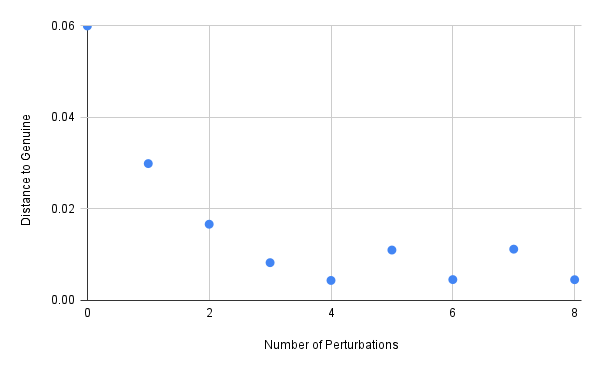
\includegraphics[width=0.8\linewidth]{dist_pert_plot.png}
    \end{center}
    \caption{Successive Perturbations on a Forgery}
    \label{fig:siamese}
\end{figure}

It appeared that the forge was just adding noise, as the genuine is noisy...
So, I did this:
$improved_forge[improved_forge < 1.0e-06] = 0.0$
...and got this:
0.06897393614053726
which is just marginally more than the distance for genuine improved\_forge
(so this background noise wasn't really helping that much)
(maybe I should count how many elements were zeroed...)


One interesting problem I ran into was I once manually saved a model just a batch or 2 after it call scheduler.step() (think it what caused it) and it performed much worse than I expected because the optimizer had made large changes... (I realized this becuase the val\_loss jumped up...)
